% Drawing 119/08-11 -- folder 119, batch 08, archive page 156 (PDF page 157).
% Transcription: icosaèdre en perspective, sommets marqués $u, u', v, v', a, b$, faces hachurées.
% Kind: icosahedron in perspective. Method 2 (schematic redraw from the facsimile). Status: partial.
% Notes: Icosahedron seen with a vertex in front: the hexagon of vertices (top T, upper right R, lower right V, bottom M = u', lower left, upper left) round the front vertices u, a, b; every edge is drawn between the same ten computed vertices. Heavy where he inked them: upper left - u, upper left - a, a - b. Edges drawn: T - upper left, T - R, u - upper left, u - R, u - b, a - b, a - upper left, a - u', b - u', b - V, R - V, upper left - lower left, lower left - u', u' - V; below, the faint lower half towards a bottom vertex: an arc from the lower left, a line from V, and a short stroke down from u' (and a short stroke down from T at the top). Hatched (as regular hatching, his is loose): the six faces round the hexagon (T-upper left-u, upper left-u-a, upper left-a-lower left, lower left-a-u', u'-b-V, b-V-R, u-R-b, T-u-R) and, faintly, the lower region; the two central faces u-a-b and a-b-u' are left blank, as on the page. A long faint curve over the top, from the left to beyond R, is drawn as a pencil curve (the old redraw closed it into an ellipse, which is not on the page). Labels as on the page: u, a, b, u', v (lower right), v' (lower left), v' (upper right, a reading); the label at the upper left (like "u?") is not readable and is left out; the faint letter under the bottom vertex, like "u", is drawn as a reading. Still differs: hatching is schematic; the two unreadable or faint labels. Redrawn 2026-11-09 (issue 128): to check again. Question settled by a machine pass on the facsimile, 2026-11-12 (page): the upper right label reads v' and the faint letter under the bottom vertex reads u; a faint u' also stands above the top vertex, just above the crop, and is now drawn, so that the labels down the axis read u', u, (a, b), u', u. Not checked by a reader.
% Coordinates: 1 unit = 1 mm = 1/100 of the crop width (bbox in page fractions: [0.12, 0.56, 0.38, 0.72]).
% Redrawn by Claude (claude-opus-5-5), issue #73, 2026-11-09; not checked by a human; not compiled (no TeX in the session).
% Rights: reproduces part of the work -- behind RENDER_TRANSCRIPTS, never published by itself.
\documentclass[tikz,border=3pt]{standalone}
\usepackage{amsmath,amssymb}
\usetikzlibrary{patterns,arrows.meta}
\tikzset{pencil/.style={black!45}, struck/.style={black!35}, mark/.style={circle,draw,inner sep=1.3pt}, pt/.style={circle,fill,inner sep=0.9pt}, opt/.style={circle,draw,fill=white,inner sep=1.1pt}}
\begin{document}
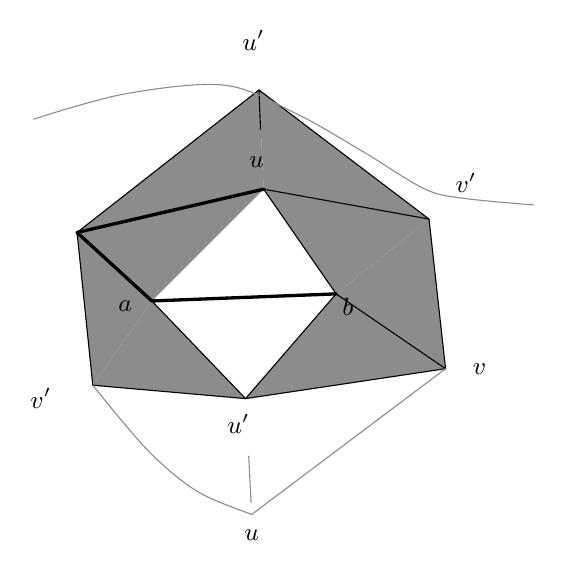
\begin{tikzpicture}[x=1mm,y=1mm,line cap=round,line join=round,font=\scriptsize]
\fill[pattern=north east lines,pencil] (60.1,-3.8) -- (37,-21.9) -- (60.7,-16.4) -- cycle;
\fill[pattern=north east lines,pencil] (37,-21.9) -- (60.7,-16.4) -- (46.5,-30.6) -- cycle;
\fill[pattern=north east lines,pencil] (37,-21.9) -- (46.5,-30.6) -- (39,-41.3) -- cycle;
\fill[pattern=north east lines,pencil] (39,-41.3) -- (46.5,-30.6) -- (58.4,-43) -- cycle;
\fill[pattern=north east lines,pencil] (58.4,-43) -- (69.9,-29.7) -- (83.8,-39.2) -- cycle;
\fill[pattern=north east lines,pencil] (69.9,-29.7) -- (83.8,-39.2) -- (81.7,-20.2) -- cycle;
\fill[pattern=north east lines,pencil] (60.7,-16.4) -- (81.7,-20.2) -- (69.9,-29.7) -- cycle;
\fill[pattern=north east lines,pencil] (60.1,-3.8) -- (60.7,-16.4) -- (81.7,-20.2) -- cycle;
\draw (60.1,-3.8) -- (37,-21.9);
\draw (60.1,-3.8) -- (81.7,-20.2);
\draw (60.7,-16.4) -- (81.7,-20.2);
\draw (60.7,-16.4) -- (69.9,-29.7);
\draw (46.5,-30.6) -- (58.4,-43);
\draw (69.9,-29.7) -- (58.4,-43);
\draw (69.9,-29.7) -- (83.8,-39.2);
\draw (81.7,-20.2) -- (83.8,-39.2);
\draw (37,-21.9) -- (39,-41.3);
\draw (39,-41.3) -- (58.4,-43);
\draw (58.4,-43) -- (83.8,-39.2);
\draw[very thick] (37,-21.9) -- (60.7,-16.4);
\draw[very thick] (37,-21.9) -- (46.5,-30.6);
\draw[very thick] (46.5,-30.6) -- (69.9,-29.7);
\draw (60.1,-3.8) -- (60.3,-8.8);
\draw[pencil] (58.8,-50.3) -- (59.1,-56.2);
\draw[pencil] plot[smooth, tension=0.55] coordinates {(39,-41.3) (46,-49.6) (52.3,-54.8) (59.2,-57.7)};
\draw[pencil] (83.8,-39.2) -- (59.2,-57.7);
\draw[pencil] plot[smooth, tension=0.55] coordinates {(31.5,-7.5) (43.1,-4.3) (55.8,-3.2) (65,-6.9) (73.1,-11.5) (81.2,-16.4) (86.4,-17.6) (95,-18.4)};
\node[inner sep=1pt] at (59.8,-13) {\small $u$};
\node[inner sep=1pt] at (59.4,2.5) {\small $u'$};
\node[inner sep=1pt] at (43.1,-31.2) {\small $a$};
\node[inner sep=1pt] at (71.4,-31.4) {\small $b$};
\node[inner sep=1pt] at (57.5,-46.2) {\small $u'$};
\node[inner sep=1pt] at (88.1,-39.2) {\small $v$};
\node[inner sep=1pt] at (32.4,-43) {\small $v'$};
\node[inner sep=1pt] at (86.4,-15.6) {\small $v'$};
\node[inner sep=1pt] at (59.2,-60.3) {\small $u$};
\end{tikzpicture}
\end{document}
